% =================================================================================================================================
% The MIT Lisence:
%
% Copyright (C) 2013 Jarmo Nikkanen
%
% Permission is hereby granted, free of charge, to any person obtaining a copy of this software and associated documentation 
% files (the "Software"), to deal in the Software without restriction, including without limitation the rights to use, copy, 
% modify, merge, publish, distribute, sublicense, and/or sell copies of the Software, and to permit persons to whom the Software 
% is furnished to do so, subject to the following conditions:
%
% The above copyright notice and this permission notice shall be included in all copies or substantial portions of the Software.
%
% THE SOFTWARE IS PROVIDED "AS IS", WITHOUT WARRANTY OF ANY KIND, EXPRESS OR IMPLIED, INCLUDING BUT NOT LIMITED TO THE WARRANTIES
% OF MERCHANTABILITY, FITNESS FOR A PARTICULAR PURPOSE AND NONINFRINGEMENT. IN NO EVENT SHALL THE AUTHORS OR COPYRIGHT HOLDERS BE
% LIABLE FOR ANY CLAIM, DAMAGES OR OTHER LIABILITY, WHETHER IN AN ACTION OF CONTRACT, TORT OR OTHERWISE, ARISING FROM, OUT OF OR
% IN CONNECTION WITH THE SOFTWARE OR THE USE OR OTHER DEALINGS IN THE SOFTWARE.
% =================================================================================================================================

\documentclass[twocolumn]{report}
\usepackage{graphicx}
\newcommand{\ident}{\indent}
\newcommand{\acos}{\cos^{-1}}
\newcommand{\asin}{\sin^{-1}}
\newcommand{\atan}{\tan^{-1}}
\newcommand{\acosh}{\cosh^{-1}}
\newcommand{\asinh}{\sinh^{-1}}
\newcommand{\ve}[1]{\overrightarrow{\mathbf{#1}}}


\setlength{\hoffset}{-0.2in} \setlength{\textwidth}{17.5cm}
\setlength{\voffset}{-0.2in}\setlength{\textheight}{21cm}

\newenvironment{twocol}[0]{%
\begin{list}{}{%
\onecolumn
\setlength{\leftmargin}{0.15cm}%
\setlength{\rightmargin}{0.15cm}%
\setlength{\topmargin}{0cm}%
\setlength{\headheight}{0cm}%
\setlength{\headsep}{0cm}%
\setlength{\textheight}{24cm}%
}%
\item[]}{\end{list}}

\begin{document}

\title{
\begin{center}
\textbf{Reflections implementation}\end{center}
\begin{center}
\textbf{For}\end{center}
\begin{center}
\textbf{D3D9Client}\end{center}
\vspace{-2cm}
}

\maketitle

\begin{twocol}

\section*{Fresnel reflection}

Fresnel reflection is probably the most common type of reflection. Good examples of material having a fresnel reflection are glass, water and most plastics. Fresnel reflection is highly depended from a viewing angle. Reflection is stronger when viewed from a shallow angle. In the D3D9Client we use so called Schlick's approximation of fresnel reflection. 

\begin{equation}
 R = R_0 + (1-R_0)(1-\cos\theta)^p
\end{equation}

Where the "Offset" $R_0$ is given by
\begin{equation}
R_0 = \left[\frac{1-n}{1+n}\right]^2
\end{equation}

To gain some additional properties for our function we have replaced the term $(1-R_0)$ with a multiplier $m$ resulting an equation

\begin{equation}
 R = R_0 + m(1-\cos\theta)^p
\end{equation}

Here are two plots of the equation using different values of $p$. Red curve is using value 2.0 and blue 4.0. The parameter $p$ will only effect in the view angle dependency of the fresnel reflection. The multiplier $m$ is most often set to a value $1-R_0$ and in that case the maximum reflection intensity is 1.0.

\begin{figure}[h]
	\centering
	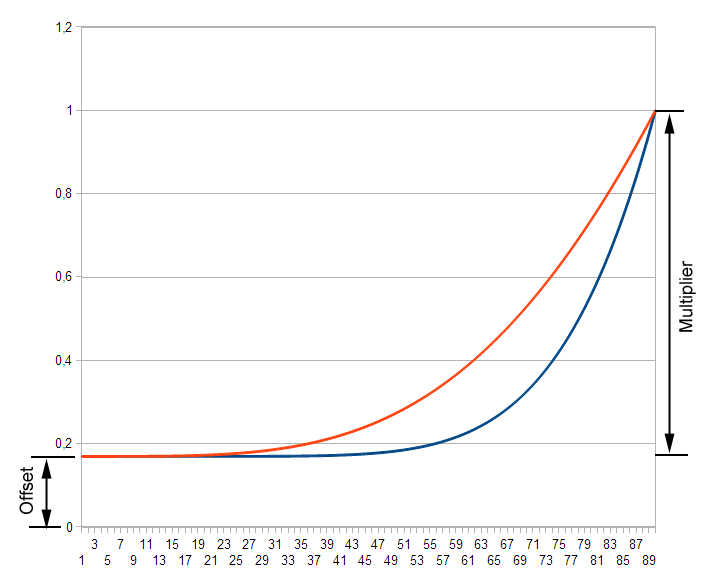
\includegraphics[width=0.6\textwidth]{images/curves.png}
	\caption{Reflection intensity as function of angle}
\end{figure}

\end{twocol}
\begin{twocol}

\section*{Reflection Model}

Here is an image about the reflection model used in D3D9Client

\begin{figure}[h]
	\centering
	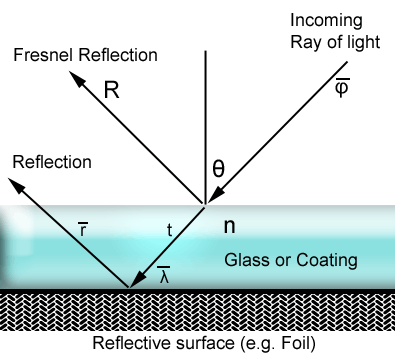
\includegraphics[width=0.35\textwidth]{images/Fresnel.png}
	\caption{Reflection model}
\end{figure}

The model consists from a fresnel reflection $R$ and a metallic reflection $r$. The lambda $\vec{\lambda}$ is a reflectivity color of the material. $t$ is a fraction of the incoming ray that is not reflected away from the interface. $\vec{\varphi}$ is the color of incoming ray of light. The value of $t$ is simply $t=1-R$.

The intensity of "metallic" reflection alone is independent from a viewing angle. However, when combined with a fresnel reflection it is given by

\begin{equation}
 \vec{r} = \vec{\lambda}(1-R)\vec{\varphi}
\end{equation}

I suppose the fresnel reflection could take a specular color $\vec{s}$ of the material but currently it is considered to be white $\vec{s}=[1,1,1]$. The total reflected light is

\begin{equation}
\vec{R_{tot}} = (\vec{\lambda}(1-R)+\vec{s}R)\vec{\varphi}
\end{equation}

The color intensity of the diffuse surface is attennuated by the reflection intensity factor $1-|\vec{\lambda}|$. Resulting pixel color $\vec{c}$ is given by following equation where $\vec{d}$ is the color of the diffuse material or a texture.

\begin{equation}
\vec{c_{rgb}} = \vec{d_{rgb}}(1-|\vec{\lambda}|) + \vec{R_{tot}}
\end{equation}

Material/Texture alpha must be modified for alpha blending stage to make reflections visible on otherwice transparent surfaces like glass. 

\begin{equation}
\vec{c_{a}} = max(\vec{d_a}, |\vec{R_{tot}}|)
\end{equation}

In the D3D9Client we simplify the computations and we do not apply fresnel equations to incoming sunlight. A diffuse surface under a reflective coating is considered to be fully lit by the sunlight and other light sources. 

If we would take the sun angle $\sigma$ in to account then the equation would become

\begin{equation}
\vec{c_{rgb}} = \vec{d_{rgb}}(1-|\vec{\lambda}|)[1-R_0-m(1-\cos\sigma)^p] + \vec{R_{tot}}
\end{equation}

\end{twocol}
\begin{twocol}

\section*{Material Editor}

Reflections are controlled by "Fresnel" and "Reflect" material properties in the material editor that is a part of D3D9Client debug controls. These properties can be used independendly from each-other or together.

\begin{figure}[h]
	\centering
	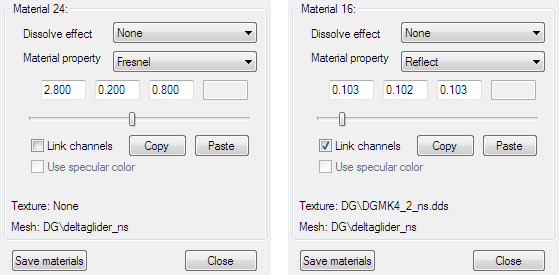
\includegraphics[width=0.45\textwidth]{images/materialed.png}
	\caption{Material Editor}
\end{figure}

\textbf{Fresnel}

The first field in fresnel parameters is the power value $p$. A typical range for the power paramater is [2.5 to 3.5]. The second field is the offset $R_0$ value and the typical range is [0.05 to 0.25]. The third field is the multiplier $m$ and the value is automatically set to 1.0-Offset when ever the offset is changed. There is usually no need to touch this value. Fresnel reflections can be disabled by setting the offset and multiplier to zero in that order.  

\textbf{Reflect}

Reflect material property is used to define metallic reflections from a materials like chrome and goldfoils. Material property fields $\vec{\lambda}$ are red, green and blue. Higher values will make the material more reflective and therefore the diffuse color is shifted towards black. Metallic reflections will be disabled if all values are set to zero. 

\textbf{Dissolve}

Dissolve is an experimental technique that can be used to create blurry or noisy reflections. Currently it can be only applied to non-normal mapped surface that has a texture. It would be possible to use a screen-space coordinates to create a similar effect to a non-textured materials as well. The first field is the effect scale factor (i.e. particle size). The second field is the effect strength. If either parameter is zero the effect will be disabled.

\textbf{Link}

The link checkbox allows the link the R, G and B fields and after that they can be adjusted simultaneously with the slider.

\textbf{Copy and Paste}

Copy and paste buttons can be used to copy RGB values from different material properties for an example from specular color to reflect color.

\end{twocol}
\end{document}
